\chapter{Evaluation}
\label{chapter:evaluation}

This chapter describes the results of taking the selected solutions into use. First the changes in selected metrics (see section \ref{section:measuring})
are presented, which is then followed by insights from the third workshop.

\section{Changes in metrics}
\label{section:metric-results}

The effectiveness of the solutions were evaluated by measuring the values of predefined metrics after the implementation phase using
exactly the same methods as in initial state analysis. The selected metrics addressed three different aspects: maintenance knowledge, maintenance process and multitasking.
Next the changes in the selected metrics are presented by comparing them to the initial values. Further implications and analysis on the goals are presented in section \ref{section:outcomes}.

\subsection{Maintenance knowledge metrics}
\label{section:knowledge-metrics-after}

Maintenance knowledge and especially sharing of it was measured with three metrics: \emph{average projects per person}, \emph{average persons per project} and \emph{significance of knowledge sharing barriers}.
The measurement was based on knowledge sharing survey initially conducted during the initial state analysis and then repeated with the same target group after the implementation phase.
To ensure validity of the results, it was confirmed that exactly the same persons responded to the survey on both times, which is necessary since the population is so small and therefore even slightly changing
the sample between measurements would render the end results invalid.

\subsubsection*{Average projects per person}

The first metric, average projects per persons on different skill and experience levels, represents the average diversity of an individual's skill set. Special interest was focused on the executives compared to
other experience levels since due to QOCO's history, the gap between the executives and other employees was initially quite significant. The results after the implementation phase are presented in
table \ref{table:projects-per-level-after} together with the change compared to the initial measurement.

\begin{table}[H]
	\begin{center}
		\begin{tabular}{|c|c|c|c|}
			\hline
            	 		& \textbf{Junior} & \textbf{Senior} & \textbf{Executive} \\ \hline
			\textbf{5}  & 2.0 (+1.0)     & 1.0 (+0.0)      & 8.3 (-1.0)          \\ \hline
			\textbf{3+} & 5.5 (+0.0)     & 3.0 (+0.0)      & 14.5 (+2.7)         \\ \hline
			\textbf{1+} & 15.3 (+0.8)    & 10.0 (+0.2)     & 22.5 (-0.3)         \\ \hline
		\end{tabular}
		
		\caption{Average amount of projects at skill level after the implementation}
		\label{table:projects-per-level-after}
	\end{center}
\end{table}

Judging by the table it is evident that junior employees have gained the most knowledge during the implementation phase, which can be seen as a 1.0 increase in level 5 knowledge and 0.8 increase in overall
knowledge at 1+ level. A significant improvement on the most detailed level 5 knowledge is mostly explained by previous level 4 knowledge that has now become level 5 due to increased confidence and overall
experience. The increase has occurred mainly on older projects that have traditionally been in the hands of the executives, but now it seems that knowledge has been shared to juniors as well.
The improvement on overall knowledge at 1+ level is partly explained by natural learning during the implementation phase, but additionally project presentations have clearly had a positive impact, since
the improvements have been larger on projects that were presented during the implementation phase.

The knowledge of the seniors on the other hand has not changed much during the implementation phase. The only difference is on the overall knowledge at 1+ level with an improvement of 0.2, which could be mostly
explained by natural learning. Another explanation is also that some knowledge has been lost while some has been gained and therefore the overall change appears as zero. Having a more detailed look on individual
answers shows that this is the case as most of the changes are between levels 1 and 3 and the increases and decreases are approximately evenly balanced.

Lastly, the executives that have traditionally had the most knowledge at QOCO have managed to maintain their position, although there is a decrease of 1.0 in level 5 knowledge. This is a result of having a high
initial value, which would require continuous effort to be maintained. Also knowledge has clearly been shared to juniors and therefore there is no need to keep knowledge at level 5 on all older projects.
On the other hand, the executives have also gained the most on 3+ level during the implementation phase, which could be explained by several older projects that have been raised from levels 1 and 2 to 3.
This has occurred due to personnel changes on the customer side, which requires the executives to revise their knowledge in order to be able to introduce the projects to new persons.
Despite revising legacy knowledge, the executives
have still lost knowledge on 1+ level, which is most likely due to natural unlearning as older projects get forgotten over time if they do not require any maintenance activities.

Analyzing the most increased and decreased projects reveals that project presentations had a positive impact on overall knowledge since all of the presented projects are in top 5 of the best known projects,
most of them with a significant increase in average knowledge level. Additionally one of the best improvements on average knowledge levels is on a project that has intentionally been shared recently to reduce
dependability on a single developer. Therefore it can be stated that the project presentations clearly have helped to increase overall knowledge throughout the company. On the other hand, it is evident that
the projects with the most lost knowledge are the ones that have been developed a while ago, but have not been recently touched. One exception to that is the Airline 1 technical operations digitalization project that
was initially the second best known project, but has lost knowledge during the implementation phase, even though it has been under continuous development. The explanation for this is most likely increasing
complexity and quite independent development process of Airline 1 development team, which effectively decreases the knowledge of those who are not actively participating on the development.

\subsubsection*{Average persons per project}

The second metric, average persons per project on different skill levels, represents the diversity of all skills sets of the organization. Even though projects per person metric would look promising, a low
average amount of persons per project would mean that the skill sets are highly focused and overlapping while leaving many projects dependent on a single person. The change in this metric is presented
in figure \ref{fig:skill-distribution-after} for easy comparison between measurements.

\begin{figure}[ht]
  \begin{center}
    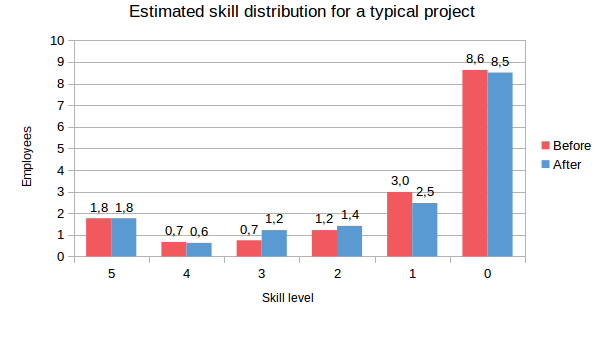
\includegraphics[width=0.9\textwidth]{images/skill-distribution-after.png}
    \caption{Estimated skill distribution for a typical project as of May 2019}
    \label{fig:skill-distribution-after}
  \end{center}
\end{figure}

As expected, 4+ level knowledge has remained mostly unchanged, since the time frame of this study was relatively short and gaining 4+ knowledge requires quite much time and effort. However, there has
been a significant improvement on level 3 knowledge, which was one of the goals for the solutions. After the implementation, there is an average increase of 0.5 persons on a typical project, which is already
a significant improvement on the previous state. Another positive fact on this metric is that the largest decrease has been on level 1, which means that knowledge of the business case has been successfully updated
to an ability to do minor tasks. Therefore it seems like the learning has occurred on various different projects, rather than being focused on a small group of projects.

\subsubsection*{Knowledge sharing barriers}

The third knowledge sharing metric, knowledge sharing barriers, aimed to identify and measure the main challenges that slow down or even entirely prevent knowledge sharing.
The most significant barriers with updated significance scores are presented below and as can be seen, the list is mostly the same as before the implementation (see section \ref{section:survey-results-before}).
Tight schedule and multitasking are still the two most significant barriers at QOCO, but their significance scores have decreased considerably. Especially tight scheduling is not as significant issue as before
since its score decreased by five points from the initial score of 15, which is a huge positive development. Both multitasking and lack of informal documentation barriers decreased by one point, which
is also positive, although not as large as that of the tight schedule barrier.

\begin{center}
	The most significant knowledge sharing barriers at QOCO after the implementation:
	
	\begin{enumerate}
		\centering
		\item Tight schedule (10)
		\item Multitasking (9)
		\item Lack of formal documentation (8)
		\item Complex domain (7)
		\item Lack of informal documentation (6)
	\end{enumerate}
\end{center}

In addition to the developments on the main focus areas, also the significance of strong code ownership decreased by three points and it has been replaced by lack of formal documentation on the list.
Lack of formal documentation has one of the largest increases in significance together with working in different locations, both of which have increased their score by three points. Lack of formal documentation
is especially interesting as the increase has ranked it to the top three of the most significant barriers after the implementation and therefore it should be addressed in the future.

\vspace{12pt}

Identifying the most significant barriers is important, but it is also important to analyze the least significant ones as well
to understand the strengths of the organization. The updated list of the least significant barriers
is presented below, and as could be expected, it is also quite similar to the initial measurement (see section \ref{section:survey-results-before}). A notable fact is that generally all of the barriers on
the previous list have increased their score by several points, which means that the barriers are even less significant than initially. The only exception is lack of motivation that has remained
unchanged with a score of 13, which is already quite high. Therefore it does not raise much concerns, although it is still worth noting.

\begin{center}
	The least significant knowledge sharing barriers at QOCO after the implementation:
	
	\begin{enumerate}
		\centering
		\item Physical work environment (17)
		\item Difference in age (17)
		\item Lack of trust (17)
		\item Strong organizational structure (16)
		\item Lack of motivation (13)
	\end{enumerate}
\end{center}

Despite the positive development on the top five list, the largest difference was on individual communication skills with an increase of nine points on its score. This was a bit surprising as the development
was so significant compared to other barriers. 
There was no single explanation for this, but it was thought to be caused by generally improved maintenance process, which simultaneously improves the overall communication.

Another interesting point on the knowledge sharing barriers is the difference in experience levels. It clearly divides opinions since it has increased its score by two on most significant and four on the least
significant barriers. By analyzing the survey responses in more detail, the explanation for this development is the difference between junior and senior employees. Two seniors selected "strongly disagree",
whereas three juniors selected "agree" and the executives were inconclusive between "agree" and "disagree". Therefore it can be argued that the seniors do not consider difference in experience levels as significant
barrier as juniors, which has many possible implications and explanations. However, based on this dataset no strong implications one way or another should be made and it should be kept in mind that it
is still quite far from the most significant barriers in terms of significance score.

\subsection{Maintenance process metrics}
\label{section:process-results}

The process itself was addressed with three metrics as well: \emph{tickets from unofficial sources}, \emph{ratio of alerts} and \emph{average resolution time}. The data source for these metrics was the data
export from Freshdesk consisting of tickets created between January and April. This period was then compared to previous export, which included the whole year of 2018.

First of all, the tickets from unofficial sources
or outside the official workflow are represented by reporter domain. The tickets that are reported through informal channels are forwarded to Freshdesk by QOCO's own employees, meaning that tickets from QOCO's domain
are from unofficial sources in most cases. Reporter domains after the implementation phase are presented in figure \ref{fig:ticket-domains-after} and as can be seen, the ratio of internally reported tickets
has actually increased to 19 \% from the initial 10 \%. The increase is also reflecting to Airline 1 domain, which has decreased by 10 percentage points after the
implementation. The proportions of other domains remain mostly unchanged with a one percentage point increase in the third party vendor domain.

\begin{figure}[ht]
  \begin{center}
    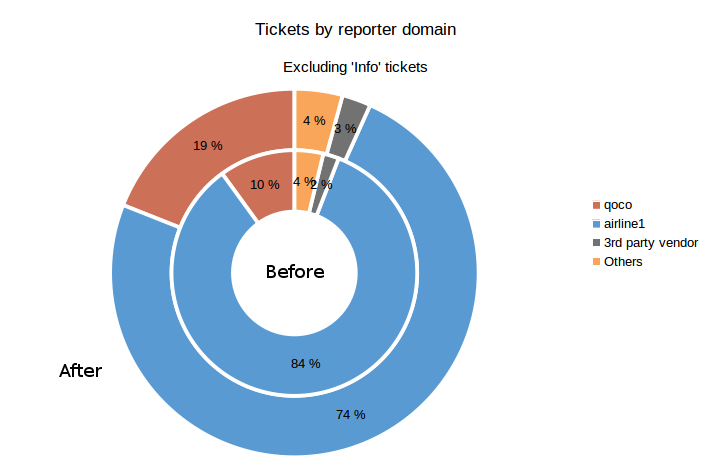
\includegraphics[width=\textwidth]{images/ticket-domains-after-2.png}
    \caption{Tickets by reporter domain after the implementation phase}
    \label{fig:ticket-domains-after}
  \end{center}
\end{figure}

The second metric, \emph{ratio of alerts}, was also interesting since it represents the automatic detection of incidents before the customer needs to report them and therefore results in a better customer
experience, but also improves the quality of incoming tickets. The distribution of ticket types after the implementation phase is presented in figure \ref{fig:ticket-types-after}. From the graph it is evident
that the ratio of alerts has decreased significantly from 7 \% to 2 \% during the implementation phase. Digging deeper into the ticket data reveals that most of the alerts in 2018 have been about network
connectivity of a single application, which has not alerted anymore between January and April. This explains the decrease in the alert ratio, but it is also worth noting that it means that there has not been many
other alerts as well, which could be a point of improvement in the future.

Another notable finding on the new distribution is an increase in request and problem tickets, although
an increase in problem tickets is most likely explained by a decrease in incident tickets since they are quite close to each other as concepts
and the total ratio of problems and incidents has not changed significantly. The reason for the increase in request tickets did not have any single explanation, but some part of the increase could be caused by
a single application requiring a bit more actions than during 2018.

\begin{figure}[ht]
  \begin{center}
    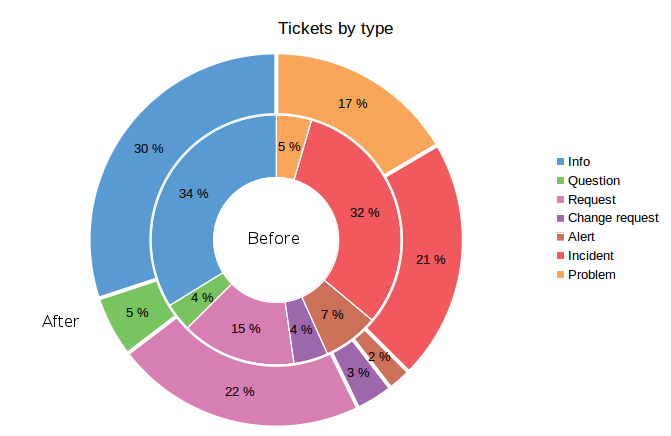
\includegraphics[width=\textwidth]{images/ticket-types-after-2.png}
    \caption{Ticket types after the implementation, excluding tickets without a type}
    \label{fig:ticket-types-after}
  \end{center}
\end{figure}

The last process metric was average resolution time as it usually directly represents customer satisfaction and maintenance process efficiency in general. The monthly average resolution time together with 
the total ticket count is presented in figure \ref{fig:resolution-times-after}. The resolution time is again plotted only for low priority tickets as they still make up 94 \% of total tickets and represent
the main process quite well. As there was only a few medium and high priority tickets, it was not meaningful to calculate the monthly average for them.

\begin{figure}[ht]
  \begin{center}
    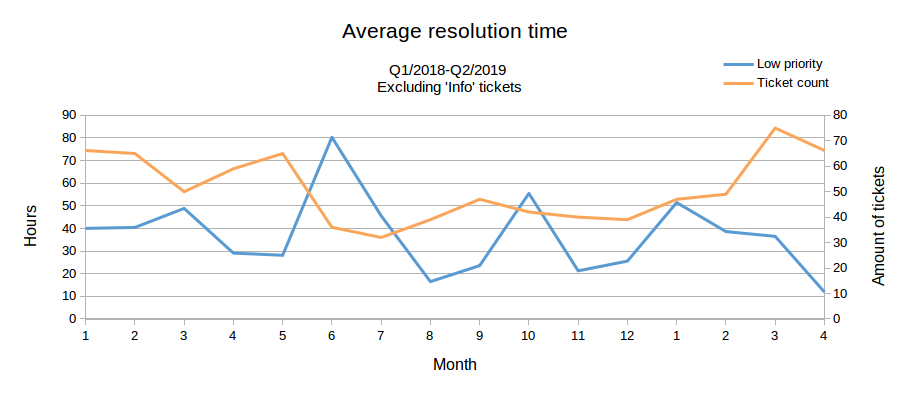
\includegraphics[width=\textwidth]{images/resolution-time-after.png}
    \caption{Average resolution times by month}
    \label{fig:resolution-times-after}
  \end{center}
\end{figure}

Judging from the graph it is evident that the average resolution time for low priority tickets has been continuing its downtrend also during the implementation phase. It is also worth noting that the average
amount of tickets created during the implementation was a record high of 70 tickets per month. This most likely means that an increasing amount of the tickets that were previously not visible in the official
process have been reported to Freshdesk either directly by the customers or forwarded by QOCO's employees. Despite this increase, it is also notable that April marks a record low for resolution times 
at approximately 12 hours on average. This is a clear sign of improvement in the process and it suggests that the solutions have managed to improve the efficiency of the maintenance process in general,
although a further confirmation is still required. Another notable thing is the presence of a periodic increase in resolution times, which was already identified during the first data export. The reason for it
remains unclear, but it is definitely something that should be further studied in the future.

\subsection{Multitasking metrics}

The last topic to be addressed was multitasking, which was measured by time tracking data with two metrics: \emph{average projects per day} and \emph{average time entries per day}. The results of the
measurement after the implementation phase are presented in table \ref{table:toggl-after} together with the change in multitasking factors compared to the initial state. As can be clearly observed from
the table, multitasking has increased during the implementation phase on almost all teams, excluding MROTools team that has remained unchanged. Also EngineData team as a new one has quite similar
multitasking levels compared to the MROTools team, which is natural since they are both product-oriented SaaS teams mainly working on a single project. What remains alarming is the fact that the Airline 1
development team had relatively high multitasking factor already before the implementation phase and it has only increased on both metrics. As already argued during the initial
phase of this study, it is worrying since an increasing amount of multitasking could lead to increased stress, lower productivity and dissatisfaction at work.

\begin{table}[H]
	\begin{center}
		\begin{tabular}{|c|c|c|}
		\hline
        		                     	  	& \textbf{Projects / day} & \textbf{Time entries / day} \\ \hline
			\textbf{Airline 1 consulting}  & 1.5 (+0.4)              & 1.8 (+0.4)                  \\ \hline
			\textbf{Airline 1 development} & 2.0 (+0.3)              & 3.5 (+0.2)                  \\ \hline
			\textbf{Executives}          	& 2.1 (+0.3)              & 2.9 (+0.5)                  \\ \hline
			\textbf{MROTools}            	& 1.1 (+0.0)              & 2.1 (+0.0)                  \\ \hline
			\textbf{EngineData}          	& 1.1 (NEW)               & 1.1 (NEW)                   \\ \hline
		
		\end{tabular}
		
		\caption{Average context switches per day after the implementation}
		\label{table:toggl-after}
	\end{center}
\end{table}

As Airline 1 development team has a high multitasking factor, which has previously varied quite much over time, it is taken into further analysis as presented in the figure \ref{fig:dev-team-toggl-after}. As
can be seen, the multitasking factor has remained mostly constant between 3.4 and 3.7, which is higher than during the first half of 2018, when it was mostly below 3.0. However, it is also notable that there has
not been as significant spikes as experienced in July-August of 2018, which adds a little bit of positivity to the overall situation. This is still a real issue that should be addressed soon to prevent
multitasking factor from increasing even further.

\begin{figure}[ht]
  \begin{center}
    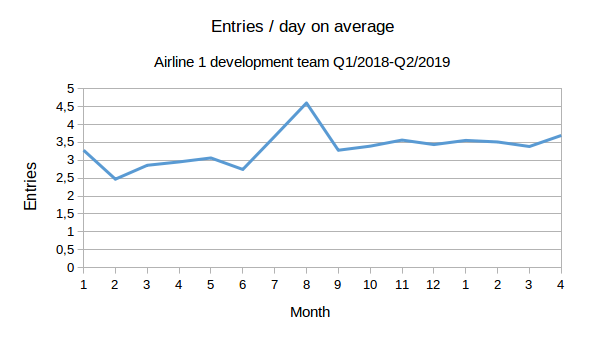
\includegraphics[width=0.9\textwidth]{images/dev-team-entries-after.png}
    \caption{Average time entries per day for Airline 1 development team}
    \label{fig:dev-team-toggl-after}
  \end{center}
\end{figure}

\section{Feedback from the third workshop}

The third workshop was organized at the end of April and its purpose was to gather quantitative data about the implemented solutions and their efficiency in solving the identified challenges.
In total there were six participants in the workshop from different development and consulting teams ensuring a wide variety of viewpoints. The workshop utilized the same
Think-Pair-Share methodology as previous ones and addressed
each of the three solutions individually.

\subsection{Triage responsibility and pair working}

The main solution in the scope of this study was considered to be rotating triage responsibility combined with pair working. It was generally complimented as a good solution to the identified challenges
and its implementation was considered generally successful. The most significant benefit of it was considered to be shared responsibility, which forces to learn about other projects and share knowledge about them.
As mentioned by the COO during the workshop, the overall feeling after the implementation phase was that rotating triage responsibility has indeed managed to reduce the workload of the CTO and COO by removing
the stress of frequently checking Freshdesk and reacting to newly created tickets. It was mutually agreed that initially it was a bit challenging to start with the newly introduced practice as knowledge
of different projects was limited and the whole process was new to all participants, but as time passed and the participants became more familiar with the support process and different projects,
also the triage responsibility became more clear.

On the practical side, the triage process was considered to be working quite well. Especially Google calendar and Slack integrations were considered useful, since they managed to integrate the triage responsibility
as a part of normal activities, rather than being just another additional process to be kept in mind. It was also identified that allocating triage responsibilities a week beforehand on a voluntary basis was
not the best solution, since it lead to several cases where finding a responsible was difficult due to vacations for example. Also allocating responsibilities on a weekly basis was considered somewhat troublesome
from the triage administrator's point of view, since he had to frequently remind people about missing allocations. In addition this, also the scalability of the process was considered, because the company aims
to be growing in the future as well. Introducing an increasing number of employees to the triage process would mean less frequent turns for each participant, which at some point is no longer practical.
Also if the company continues to grow its business, also the ticket amount will most likely increase, which is no longer maintainable by a single triage responsible at some point. However, these are still
challenges of the future and it was considered that the current model works well at least for now, although the future challenges are good to keep in mind.

Another challenge that was not initially considered was the amount of old tickets that are still unresolved after several months. Although this is not directly related to triaging incoming tickets, it was
considered that the responsibility to check these should be added to the triage responsibilities. This would ensure that they do not get forgotten and that Freshdesk is actually representing the overall state
of the maintenance process and does not get flooded with old tickets.

Pair working as a part of the triage process was also used a few times, although not nearly as much as was initially thought. When it was used it was considered helpful and fulfilling its purpose, but its
implementation was still considered challenging. This was mostly because many of the incoming tickets require access to different AMOS or cloud environments, which is a highly limiting factor. As these
accesses are managed by the customers and they can not be shared to the whole organization for security reasons, it is inconvenient to use pair working on tickets that can only be resolved with specific access
rights.

To conclude the findings related to triage and pair working process, it was agreed that the triage process should continue after the implementation phase as well. The overall process was considered to be working
well and serving its purpose, but two minor changes was added to it after the discussion. First of all, the triage turns are no longer allocated on a voluntary basis as it was considered problematic. The new 
practice on allocating turns is that the triage administrator assigns the responsibilities for the next month onwards by using Google calendar invites. This ensures that all days are assigned well beforehand
and reduces the stress related to allocations. Secondly the responsibility to check old unresolved tickets was added for the triage responsible to ensure that Freshdesk actually represents the state of
maintenance process accurately. Pair working was also considered as a good practice that could continue in the future, but it was agreed that it requires further discussions to make it meaningful and more
beneficial.

\subsection{README template}

The solution to improve the quality and quantity of informal documentation was to create a general README template for QOCO that could be used in all projects as a general guideline. The template itself was considered
useful and it was added to 17 projects in total, which is a significant amount, although it does not include every single project in an active development phase. One of the main contradictions on
writing README files was considered to be the fact that they should be written when they are needed the least, meaning that the README file should be written when the project is under active development even though
it might not be needed then. This leads to writing README files being considered as boring and unnecessary, which leads to low quality documentation. It was also discussed that updating and maintaining these files
and the template itself is somewhat challenging and easily forgotten, which decreases the benefit of them, as they might get outdated easily.

Another discussion related to the README template and the files in general raised a question about the role of a README file compared to other documentation tools that are also in use. It could be stated that the
documentation practices at QOCO are still under development and therefore the relationship between different tools for documentation is still unclear, which is a topic to be addressed in the near future. It was still
agreed that the README template should be used at least for now, but it was also pointed out that an even more important aspect to be improved in the near future should be unified practices of software
lifecycle management, including handover practices and documentation. The README template could be included in these practices as an important part or it could be replaced with a more formal documentation,
but either way, the practices should be mutually agreed and implemented.

\subsection{Project presentations}

In addition to two other solutions, project presentations were also added as a supportive solution to improve knowledge sharing. They raised a lot of discussion during the workshop and it was mutually agreed
that the project presentations were considered interesting and useful. The most important benefit of them was naturally knowledge sharing as intended, but also practicing presentation skills was considered
a positive side effect since they are constantly required during the customer meetings for example. It seemed that the presentation topics were selected correctly since all of them received positive feedback
and it was considered interesting to learn about different projects across the team boundaries. As the presentations were arranged during the casual Friday meetings, the presentations had a wide audience
and a relaxed atmosphere, which was deemed as something to be continued in the future as well.

The challenges of the project presentations were mainly around the selection of topics and scheduling. There were quite a few suggestions about future topics related to different parts of AMOS for example, which is
still a relatively unknown field for many employees. On the scheduling side it was noted that a weekly presentation is maybe a bit too much, but the schedule should not be too loose either. Therefore
at least a monthly cycle was suggested and generally considered as a balanced option, which still leaves the schedule open for more presentations if there is a natural spot to have one, after a release
for example.

Additional challenge of short presentations was considered to be focusing since a short and concise presentation could not cover much of the details of a larger topic. Many of the presentations
exceeded the loose time limit of 10 minutes even though they were not that detailed and therefore it is a challenge to be kept in mind. It is mostly tackled by a careful selection of the topics, which would
also keep the preparation time reasonable, because the purpose is not to give a detailed 1-hour presentation on different projects.

\vspace{12pt}

To conclude the feedback from the last workshop, all of the implemented solutions were generally considered as good and they managed to address the identified challenges properly.
All of the solutions will continue after this study as well with some minor changes to practicalities. They also raised some discussion about
future challenges of them and the organization in general, which acts as a starting point for the next iteration of improvements.